\section{wg\_\-wrapper Class Reference}
\label{classwg__wrapper}\index{wg_wrapper@{wg\_\-wrapper}}
Collaboration diagram for wg\_\-wrapper:\begin{figure}[H]
\begin{center}
\leavevmode
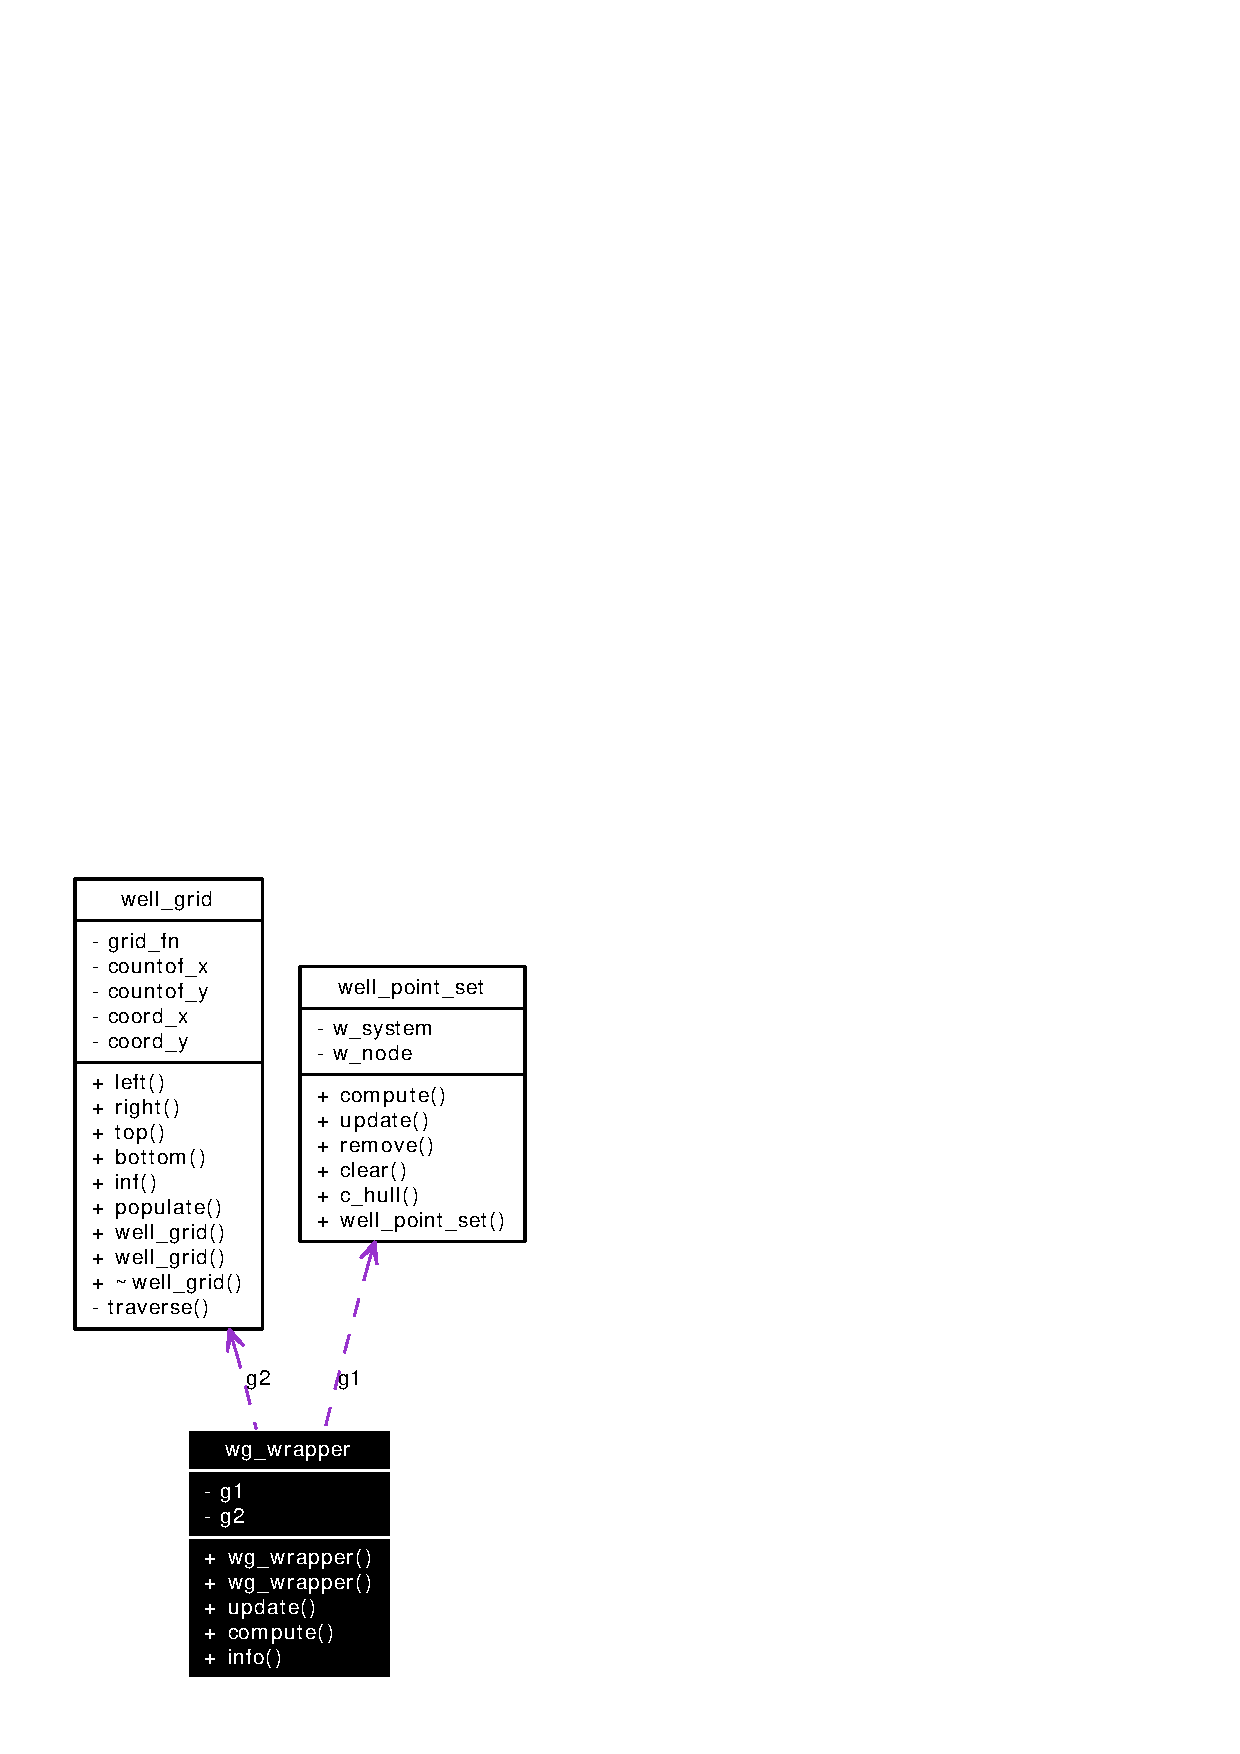
\includegraphics[width=126pt]{classwg__wrapper__coll__graph}
\end{center}
\end{figure}
\subsection*{Public Types}
\begin{CompactItemize}
\item 
typedef {\bf well\_\-point\_\-set::split\_\-func} {\bf split\_\-func}\label{classwg__wrapper_w0}

\end{CompactItemize}
\subsection*{Public Member Functions}
\begin{CompactItemize}
\item 
{\bf wg\_\-wrapper} (int cx, int cy, double x1, double x2, double y1, double y2)\label{classwg__wrapper_a0}

\item 
{\bf wg\_\-wrapper} (int cx, int cy, double $\ast$init\_\-x, double $\ast$init\_\-y)\label{classwg__wrapper_a1}

\item 
void {\bf update} (const {\bf well\_\-type} $\ast$w)\label{classwg__wrapper_a2}

\item 
void {\bf compute} ({\bf split\_\-func} fn)\label{classwg__wrapper_a3}

\item 
double {\bf info} (const {\bf well\_\-type} $\ast$w, int x, int y) const \label{classwg__wrapper_a4}

\end{CompactItemize}


\subsection{Detailed Description}




Definition at line 1051 of file wellgrid.cpp.

The documentation for this class was generated from the following file:\begin{CompactItemize}
\item 
wellgrid.cpp\end{CompactItemize}
